\documentclass[aps,pre,twocolumn,superscriptaddress,floatfix]{revtex4-2}
\usepackage{amsmath,amssymb,graphicx,bm}

\newcommand{\Dz}{\mathcal{D}z}

\begin{document}

\title{Large-deviation quasipotential for sequence retrieval in dense associative memories}

\author{Joel D. Eaves}
\affiliation{Department of Chemistry, University of Colorado Boulder, Boulder, Colorado 80309, USA}

\begin{abstract}
The retrieval overlap $M$ of a dense associative memory that recalls a sequence of patterns under synchronous dynamics obeys a stochastic one-dimensional map with noise of order $N^{-1/2}$. The dynamics has no energy function, so a free energy cannot be used to decide which of two coexisting attractors is stable. We derive the large-deviation rate function for the transitions of $M$ and the quasipotential $W$ that it generates, and we compare $W$ with the quasipotential $V$ of the Fokker-Planck approximation. For $p=2$ and $p=3$ body interactions, we compute the spinodal and the binodal in the plane of temperature and memory load. The Fokker-Planck binodal lies within $0.016\,\alpha_c$ of the large-deviation binodal at all temperatures.
\end{abstract}

\maketitle

\section{Stochastic map for the overlap}

We consider $N$ Ising spins with $p$-body couplings \cite{AbbottArian1987,KrotovHopfield2016} built from $P=\alpha N^{p-1}$ random patterns, in which the field generated by pattern $\mu$ points along pattern $\mu+1$ \cite{SompolinskyKanter1986}. All spins update in parallel \cite{Little1974} at temperature $T=1/\beta$. Let $M_t$ be the overlap of the configuration at step $t$ with the pattern being recalled at that step. In dynamical mean-field theory, the aligned spin $x_i=\xi_i^{\mu+1}s_i(t+1)=\pm1$ at site $i$ has conditional mean $\tanh\beta[M_t^{p-1}/(p-1)!+\eta_i]$, where the crosstalk fields $\eta_i$ are Gaussian with variance $\sigma^2=\alpha\rho/(p-1)!$ and are independent across sites and across time steps. The factor $\rho$ equals one for $p\ge3$. For $p=2$, $\rho=[1-\beta^2(1-\tilde q)^2]^{-1}$ with $\tilde q=\int\!\Dz\,\tanh^2\beta(M+\sigma z)$, where $\Dz$ is the standard Gaussian measure. After the average over $\eta_i$, the $x_i$ are independent and identically distributed with mean
\begin{equation}
F(M)=\int\!\Dz\,\tanh\beta\!\left[\frac{M^{p-1}}{(p-1)!}+\sigma z\right],
\label{eq:F}
\end{equation}
and the overlap at the next step is their average, $M_{t+1}=N^{-1}\sum_i x_i$. The deterministic map $M_{t+1}=F(M_t)$ has a disordered fixed point at $M=0$ and, below the spinodal, a retrieval fixed point $m^*$ and an unstable fixed point $m_s$ between them.

\section{Rate function and quasipotential}

Given $M_t=M$, the scaled cumulant generating function of $M_{t+1}$ is
\begin{equation}
\Lambda_M(\lambda)=\frac1N\ln\left\langle e^{\lambda N M_{t+1}}\right\rangle=\ln\left[\cosh\lambda+F(M)\sinh\lambda\right],
\label{eq:scgf}
\end{equation}
which holds at any temperature because $x_i^2=1$. Cram\'er's theorem \cite{Touchette2009} then gives the transition probability $P(M'|M)\asymp\exp[-N I(M'|M)]$, where the rate function is the Legendre transform of $\Lambda_M$,
\begin{equation}
I(M'|M)=\sum_{s=\pm1}\frac{1+sM'}{2}\ln\frac{1+sM'}{1+sF(M)}.
\label{eq:rate}
\end{equation}
Equation~\eqref{eq:rate} is the relative entropy of a binary variable with mean $M'$ with respect to one with mean $F(M)$. It vanishes only on the deterministic map, $M'=F(M)$, and its curvature there is the inverse of the variance $D(M)=1-F(M)^2$.

The overlap is a Markov chain, so a path has probability
\begin{equation}
P[M_0,\dots,M_n]\asymp\exp\Big[-N\sum_{t=0}^{n-1}I(M_{t+1}|M_t)\Big].
\label{eq:path}
\end{equation}
Following Freidlin and Wentzell \cite{FreidlinWentzell,Kifer1988}, we define the quasipotential relative to an attractor $a$ as the least action over paths of any length that start at $a$,
\begin{equation}
W_a(M)=\inf_{n}\;\inf_{M_0=a,\;M_n=M}\;\sum_{t=0}^{n-1}I(M_{t+1}|M_t).
\label{eq:W}
\end{equation}
It satisfies the dynamic programming equation
\begin{equation}
W_a(M')=\min_{M}\left[W_a(M)+I(M'|M)\right],\qquad W_a(a)=0,
\label{eq:bellman}
\end{equation}
which is also the stationarity condition of the chain at leading exponential order within the basin of $a$. Motion along the deterministic map costs nothing, so $W_a$ cannot increase along a deterministic trajectory.

The mean time to leave the disordered state grows as $\exp[N W_0(m^*)]$, and the mean time to leave the retrieval state grows as $\exp[N W_{m^*}(0)]$. Balance of the probability flux between the two basins gives the ratio of stationary weights,
\begin{equation}
\frac{\pi(m^*)}{\pi(0)}\asymp\exp\left\{N\left[W_{m^*}(0)-W_0(m^*)\right]\right\}.
\label{eq:ratio}
\end{equation}
Retrieval is the stable state when $W_{m^*}(0)>W_0(m^*)$ and is metastable otherwise. The binodal is the locus
\begin{equation}
W_0(m^*)=W_{m^*}(0),
\label{eq:binodal}
\end{equation}
and the spinodal is the saddle-node bifurcation of the map, $F(m)=m$ and $F'(m)=1$. The spinodal depends on the drift alone, but the binodal requires both quasipotentials, each computed from its own attractor. A single quasipotential computed from $M=0$ gives the cost to reach $m^*$ and says nothing about how long the system remains there.

\section{Relation to the Fokker-Planck quasipotential}

The Fokker-Planck description follows from Eq.~\eqref{eq:rate} in two steps. Truncation of $I$ at second order in $M'-F(M)$ gives Gaussian transitions with variance $D(M)/N$. If the drift $f(M)=F(M)-M$ is also small enough that $M$ changes little in one step, the chain becomes a diffusion, $\partial_tP=-\partial_M(fP)+(2N)^{-1}\partial_M^2(DP)$, and the ansatz $P\asymp e^{-NV}$ gives
\begin{equation}
V'(M)=-\frac{2f(M)}{D(M)}.
\label{eq:V}
\end{equation}
In one dimension $V$ is a single function, and the binodal condition is $V(m^*)=V(0)$. Equation~\eqref{eq:V} neglects the third and higher cumulants of Eq.~\eqref{eq:scgf} and the discreteness of the time step, and for master equations these approximations are known to change the exponent of the escape rate \cite{HanggiGrabert1984}. Both approximations become exact as $f\to0$ on the interval between the attractors. They do not affect the fixed points or their stability, so the spinodal is the same in the two descriptions.

\section{Results}

We solved Eq.~\eqref{eq:bellman} by a shortest-path search \cite{Dijkstra1959} on a uniform grid of 1001 points on $0\le M\le1$ for $p=3$ and 501 points for $p=2$, with the fixed point $m^*$ added as a node. At $p=3$, $T=0.1$, and $\alpha=0.09$, both barriers changed by less than $0.1\%$ between 501 and 2001 points. We evaluated the Gaussian integrals by the trapezoid rule with spacing $\Delta z=0.004$, because Gauss-Hermite quadrature with 80 nodes produced spurious discontinuities in $F$ for $p=2$ at low temperature. Figure~\ref{fig:phase} shows the spinodal and the two binodals, with the load scaled by the spinodal load at zero temperature, $\alpha_c=0.2691$ for $p=2$ and $\alpha_c=0.1261$ for $p=3$.

\begin{figure*}[t]
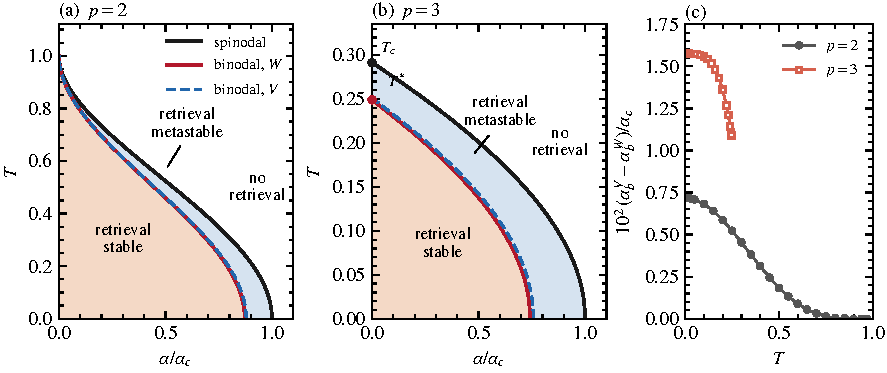
\includegraphics[width=\textwidth]{fig_phase.pdf}
\caption{Spinodal and binodal of the retrieval state for (a) $p=2$ and (b) $p=3$. The load $\alpha$ is scaled by the spinodal load at $T=0$, $\alpha_c$. The solid red line is the binodal from the large-deviation quasipotential, Eq.~\eqref{eq:binodal}, and the dashed blue line is the binodal from the Fokker-Planck quasipotential, Eq.~\eqref{eq:V}. Retrieval is metastable between the binodal and the spinodal. In (a) the curves were computed for $T\le0.97$ and are drawn to $\alpha=0$ at $T=1$. In (b) the binodal ends at $T^*$ and the spinodal ends at $T_c$. (c) Difference between the two binodal loads, in units of $10^{-2}\alpha_c$.}
\label{fig:phase}
\end{figure*}

For $p=3$ at $T=0$, the binodal is at $\alpha_b^W=0.0935$ from Eq.~\eqref{eq:binodal} and at $\alpha_b^V=0.0955$ from Eq.~\eqref{eq:V}, or $0.742\,\alpha_c$ and $0.758\,\alpha_c$. The retrieval fixed point exists at $\alpha\to0$ for $T<T_c=\max_m m^2/(2\tanh^{-1}m)=0.2913$, but $F'(0)=0$ at any load, so the disordered state remains attracting and its barrier $W_0(m^*)$ remains finite as $\alpha\to0$. The binodal therefore ends at a lower temperature, $T^*=0.249$ from $W$ and $T^*=0.251$ from $V$, and for $T^*<T<T_c$ retrieval is metastable at every load at which it exists. We obtained $T^*$ by linear extrapolation of the binodal to $\alpha=0$.

For $p=2$ at $T=0$, $\alpha_b^W=0.2346$ and $\alpha_b^V=0.2365$, or $0.872\,\alpha_c$ and $0.879\,\alpha_c$. The ratio of the binodal load to the spinodal load at the same temperature decreases from $0.872$ at $T=0$ to $0.743$ at $T=0.97$, the highest temperature computed. We found a binodal at every temperature at which we found a spinodal, in contrast to $p=3$.

The difference between the two binodals [Fig.~\ref{fig:phase}(c)] is largest at $T=0$, where it is $0.016\,\alpha_c$ for $p=3$ and $0.007\,\alpha_c$ for $p=2$. For $p=2$ it falls below $10^{-4}\alpha_c$ for $T\ge0.8$, where $m^*$ and therefore $f$ are small, which is consistent with the conditions for Eq.~\eqref{eq:V} stated above. The Fokker-Planck quasipotential therefore locates the binodal to within $2\%$ of $\alpha_c$ in both models, although the barriers themselves need not agree to the same accuracy away from the binodal.

Two assumptions underlie these results. Equation~\eqref{eq:rate} holds at the level of dynamical mean-field theory, in which the crosstalk fields are independent across sites and time steps. For $p=2$, the expression for $\rho$ is derived at a fixed point of the map, and we have used it at all $M$. A simulation of the $N$-spin network at $p=2$ would test that extrapolation, and we have not performed one.

\begin{thebibliography}{9}
\bibitem{AbbottArian1987} L. F. Abbott and Y. Arian, Storage capacity of generalized networks, Phys. Rev. A \textbf{36}, 5091 (1987).
\bibitem{KrotovHopfield2016} D. Krotov and J. J. Hopfield, Dense associative memory for pattern recognition, in \textit{Advances in Neural Information Processing Systems} \textbf{29} (2016).
\bibitem{SompolinskyKanter1986} H. Sompolinsky and I. Kanter, Temporal association in asymmetric neural networks, Phys. Rev. Lett. \textbf{57}, 2861 (1986).
\bibitem{Little1974} W. A. Little, The existence of persistent states in the brain, Math. Biosci. \textbf{19}, 101 (1974).
\bibitem{Touchette2009} H. Touchette, The large deviation approach to statistical mechanics, Phys. Rep. \textbf{478}, 1 (2009).
\bibitem{FreidlinWentzell} M. I. Freidlin and A. D. Wentzell, \textit{Random Perturbations of Dynamical Systems}, 3rd ed. (Springer, Berlin, 2012).
\bibitem{Kifer1988} Y. Kifer, \textit{Random Perturbations of Dynamical Systems} (Birkh\"auser, Boston, 1988).
\bibitem{HanggiGrabert1984} P. H\"anggi, H. Grabert, P. Talkner, and H. Thomas, Bistable systems: Master equation versus Fokker-Planck modeling, Phys. Rev. A \textbf{29}, 371 (1984).
\bibitem{Dijkstra1959} E. W. Dijkstra, A note on two problems in connexion with graphs, Numer. Math. \textbf{1}, 269 (1959).
\end{thebibliography}

\end{document}
